\chapter{Analyse}

\section{Augmented Reality Frameworks}

\cite{Poth2017} Vergleichende Studie mit Bezug zu IOT, Evaluierung der Augmented Reality Frameworks erfolgt anhand des Business Readiness Rating (BRR) Modells,
Für die Vorauswahl nimmt sie die Kritärien  a) Freie Entwicklungslizenz: b) Cross-Plattform: c) Natural Feature Tracking: und wählt 5 Frameworks aus 40. 
Bei den anderen Frameworks kommt sie zur folgenden Entscheidungsmatrix:  

Grad Kategorie Gewichtung
1 Functionality 30 %
2 Quality 25 %
3 Documentation 20 %
4 Community 10 %
5 Usability 5 %
6 Adoption 5 %
7 Support 5 %


%ARKit?

%Vuforia: Unterstützt AR Core, AR Kit also Plattformunabhägingkeit für mobile Engeräte. Wikitude auch!
% VisionLib: CAD basiertes 3D Objekterkennung und Vervolgung. Edge Tracking. Lichtverhältnisse, wenig Textur, 

\section{Annotationen in AR}

\cite{Brandenburg2019}

\section{Zeigen und Auswählen in AR Benutzeroberflächen}

% Vorgang: 

\section{Kundenintegration}

%Definition und Grobkonzept

\begin{figure}[H]
	\centering
	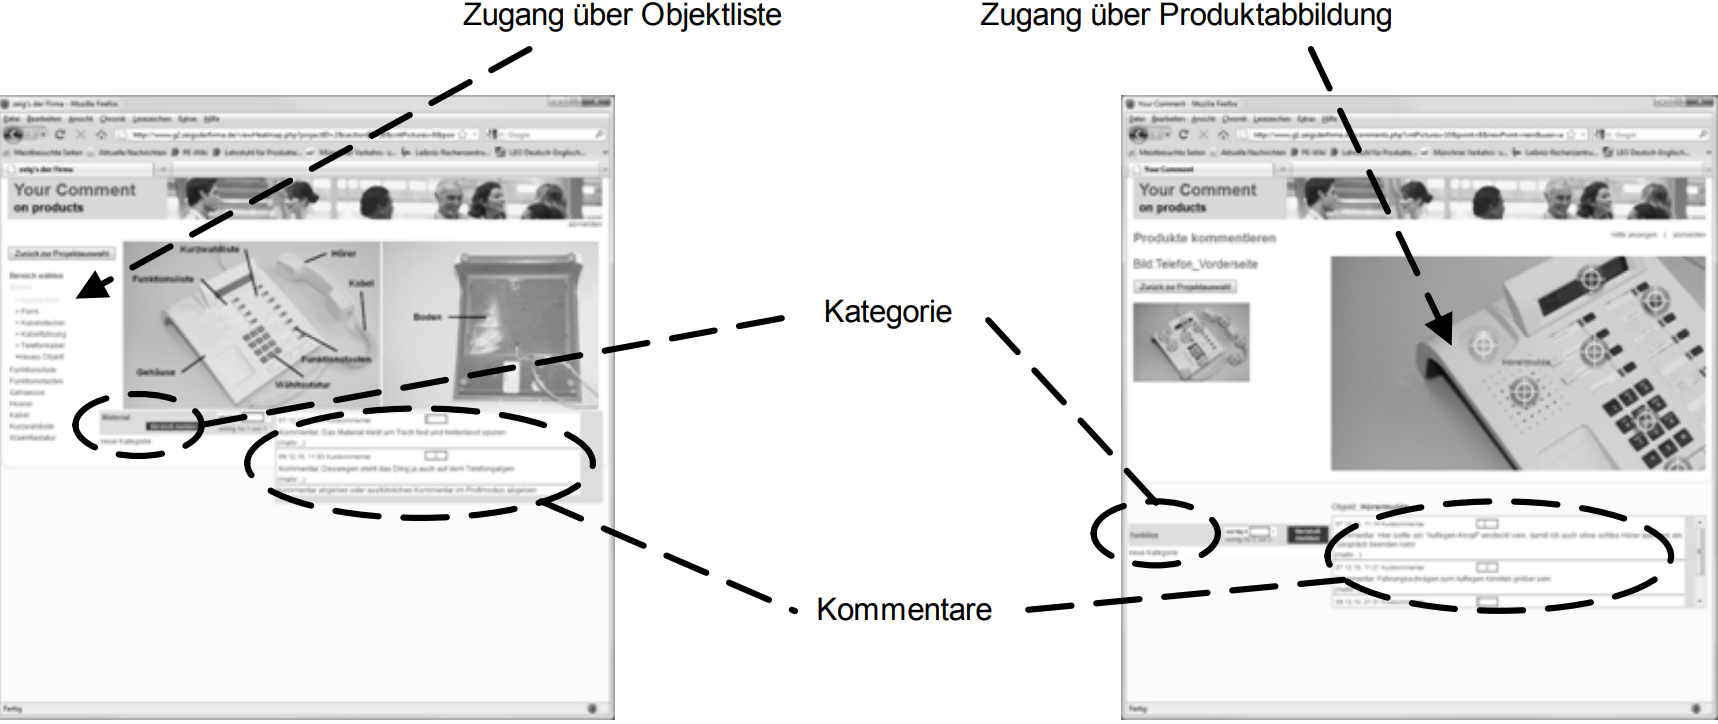
\includegraphics[width=1.0\textwidth]{resources/analyse/IPI_Vergleich_Listen_BildAnnotationeAnsicht.png}
	\caption{Online-Produktkommentierung über Listen- und Bildzugang. Quelle: \cite[S.~7]{Kirschner2011}}
	\label{img:ipi_list_image}
\end{figure}

\begin{figure}[H]
	\centering
	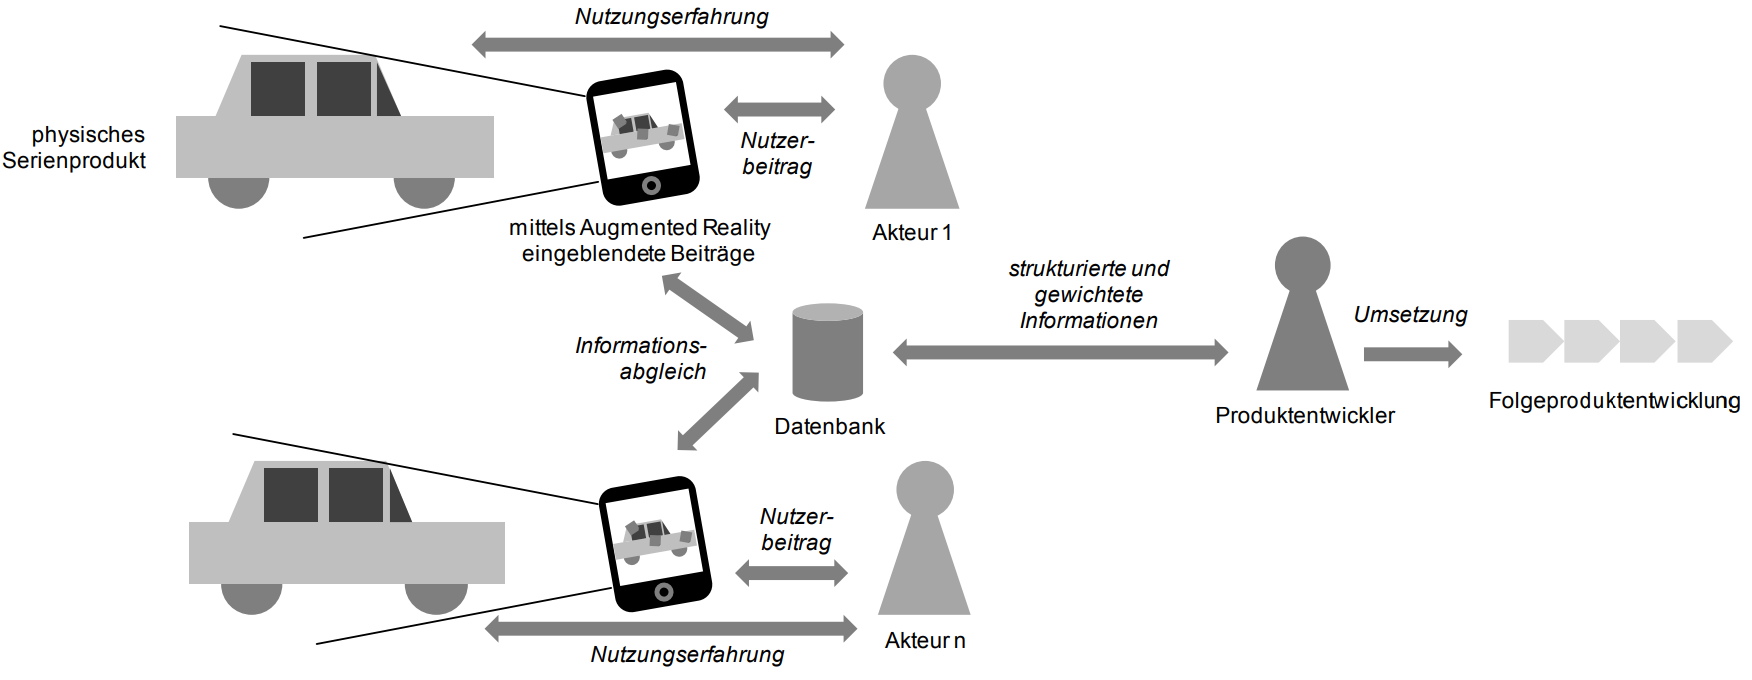
\includegraphics[width=1.0\textwidth]{resources/analyse/IPI_Objektzentriert.png}
	\caption{Informationsfluss  in der objektzentrierten IPI-Umsetzung. Quelle:\cite[S.~135]{Kirschner2012}}
	\label{img:objekt_centered_ipi}
\end{figure}


%kurz pysische 

%Bildzentriert. Vergleich mit Liste. Ergebnisse der Studie aus 2011

% Objektzentriert.

\section{Zusammenfassung}